% Options for packages loaded elsewhere
\PassOptionsToPackage{unicode}{hyperref}
\PassOptionsToPackage{hyphens}{url}
%
\documentclass[
  11pt,
]{article}
\usepackage{amsmath,amssymb}
\usepackage{iftex}
\ifPDFTeX
  \usepackage[T1]{fontenc}
  \usepackage[utf8]{inputenc}
  \usepackage{textcomp} % provide euro and other symbols
\else % if luatex or xetex
  \usepackage{unicode-math} % this also loads fontspec
  \defaultfontfeatures{Scale=MatchLowercase}
  \defaultfontfeatures[\rmfamily]{Ligatures=TeX,Scale=1}
\fi
\usepackage{lmodern}
\ifPDFTeX\else
  % xetex/luatex font selection
    \setmainfont[]{Times New Roman}
\fi
% Use upquote if available, for straight quotes in verbatim environments
\IfFileExists{upquote.sty}{\usepackage{upquote}}{}
\IfFileExists{microtype.sty}{% use microtype if available
  \usepackage[]{microtype}
  \UseMicrotypeSet[protrusion]{basicmath} % disable protrusion for tt fonts
}{}
\makeatletter
\@ifundefined{KOMAClassName}{% if non-KOMA class
  \IfFileExists{parskip.sty}{%
    \usepackage{parskip}
  }{% else
    \setlength{\parindent}{0pt}
    \setlength{\parskip}{6pt plus 2pt minus 1pt}}
}{% if KOMA class
  \KOMAoptions{parskip=half}}
\makeatother
\usepackage{xcolor}
\usepackage[margin=1in]{geometry}
\usepackage{graphicx}
\makeatletter
\def\maxwidth{\ifdim\Gin@nat@width>\linewidth\linewidth\else\Gin@nat@width\fi}
\def\maxheight{\ifdim\Gin@nat@height>\textheight\textheight\else\Gin@nat@height\fi}
\makeatother
% Scale images if necessary, so that they will not overflow the page
% margins by default, and it is still possible to overwrite the defaults
% using explicit options in \includegraphics[width, height, ...]{}
\setkeys{Gin}{width=\maxwidth,height=\maxheight,keepaspectratio}
% Set default figure placement to htbp
\makeatletter
\def\fps@figure{htbp}
\makeatother
\setlength{\emergencystretch}{3em} % prevent overfull lines
\providecommand{\tightlist}{%
  \setlength{\itemsep}{0pt}\setlength{\parskip}{0pt}}
\setcounter{secnumdepth}{-\maxdimen} % remove section numbering
% definitions for citeproc citations
\NewDocumentCommand\citeproctext{}{}
\NewDocumentCommand\citeproc{mm}{%
  \begingroup\def\citeproctext{#2}\cite{#1}\endgroup}
\makeatletter
 % allow citations to break across lines
 \let\@cite@ofmt\@firstofone
 % avoid brackets around text for \cite:
 \def\@biblabel#1{}
 \def\@cite#1#2{{#1\if@tempswa , #2\fi}}
\makeatother
\newlength{\cslhangindent}
\setlength{\cslhangindent}{1.5em}
\newlength{\csllabelwidth}
\setlength{\csllabelwidth}{3em}
\newenvironment{CSLReferences}[2] % #1 hanging-indent, #2 entry-spacing
 {\begin{list}{}{%
  \setlength{\itemindent}{0pt}
  \setlength{\leftmargin}{0pt}
  \setlength{\parsep}{0pt}
  % turn on hanging indent if param 1 is 1
  \ifodd #1
   \setlength{\leftmargin}{\cslhangindent}
   \setlength{\itemindent}{-1\cslhangindent}
  \fi
  % set entry spacing
  \setlength{\itemsep}{#2\baselineskip}}}
 {\end{list}}
\usepackage{calc}
\newcommand{\CSLBlock}[1]{\hfill\break\parbox[t]{\linewidth}{\strut\ignorespaces#1\strut}}
\newcommand{\CSLLeftMargin}[1]{\parbox[t]{\csllabelwidth}{\strut#1\strut}}
\newcommand{\CSLRightInline}[1]{\parbox[t]{\linewidth - \csllabelwidth}{\strut#1\strut}}
\newcommand{\CSLIndent}[1]{\hspace{\cslhangindent}#1}
\usepackage{setspace}\singlespacing
\usepackage{wrapfig}
\usepackage[singlelinecheck=false]{caption}
\usepackage{caption}
\captionsetup[figure]{font=small}
\pagenumbering{gobble}
\ifLuaTeX
  \usepackage{selnolig}  % disable illegal ligatures
\fi
\usepackage{bookmark}
\IfFileExists{xurl.sty}{\usepackage{xurl}}{} % add URL line breaks if available
\urlstyle{same}
\hypersetup{
  pdftitle={Review of the Literature on Oyster Bed Microbial Communities},
  pdfauthor={Kelly Miller},
  hidelinks,
  pdfcreator={LaTeX via pandoc}}

\title{Review of the Literature on Oyster Bed Microbial Communities}
\author{Kelly Miller}
\date{2025-02-07}

\begin{document}
\maketitle

\section{Introduction to the microbial
world}\label{introduction-to-the-microbial-world}

Microorganisms are the unsung heroes of primary production In a
narrative that usually centers around plants. They work on a scale we
cannot see, but the effects of their cumulative efforts are impossible
to miss; half of the oxygen in each breath we take has been produced by
oceanic microbes (Pomeroy et al., n.d.). Take a breath. (Thanks
microbes!)

Let's start with meeting the three domains of life: Bacteria, Archaea,
and Eukarya. In the classification system (\emph{i.e.} domain, kingdom,
phylum, and species), domain is the broadest level of distinction.
Humans belong to Eukarya, along with plants, fungi, and many microbial
speciesIn other words, in the most basic delineation between life forms
present on Earth, we, in all of our complexity, are grouped with plants,
fungi, and many microbial species (including some single-celled
microbes), while the two remaining categories are not only exclusively
microbes, but exclusively prokaryotic\footnote{Prokaryotes: Unicellular
  microbes with free-floating genetic material in their cytoplasm. They
  can have organelles, like ribosomes (which all organisms have) or
  flagella (little extracellular hairlike-structures that enable
  movement for cells), but they do not have membrane-bound organelles. A
  prokaryotic cell is like DNA/RNA-cytoplasm soup.} m

There is incredible biodiversity and functional diversity in the
microbial world. Our genus (\emph{Homo}) contains our species
(\emph{Homo sapien}) and our extinct primate ancestors (ex. \emph{Homo
erectus}). Compare this to the bacterial genus \emph{Streptococcus},
which includes bacteria that ferment milk into cheese and yogurt, live
in soil, populate and help regulate several of our organ systems, and
can cause strep throat and scarlet fever--among other bacterial
infections. All of this within one clade of bacteria.

Instead of performing metabolic pathways from start to finish, like the
way our digestive systems pass food from mouth to esophagus to stomach
to small intestine, etc., microorganisms are reliant on each other to
achieve comparable biological processes. Take a look at the
denitrification step of the nitrogen cycle, which--among other
applications--is facilitated by microbial communities in the marine
sediments associated with oyster farms: nitrate
(NO\textsubscript{3}\textsuperscript{-}) is converted to nitrite
(NO\textsubscript{2}\textsuperscript{-}) which is converted to nitric
oxide (NO) and then to nitrous oxide (N\textsubscript{2}O) and finally
to dinitrogen (N\textsubscript{2}). The diagram below shows the equation
for denitrification, as well as the enzyme that catalyzes each step of
the pathway (ex. nitrate reductase) and the gene responsible for that
particular enzyme (ex. \emph{Nar}) ({``Denitrifying Bacterium - an
Overview \textbar{} ScienceDirect Topics,''} n.d.) . I depict
denitrification as a linear process, although it is truly one component
of the cyclical path in which nitrogen flows through ecosystems--a.k.a.
the nitrogen cycle.

\textbf{\^{}\^{}\^{}``intermediate microbial pathways}''

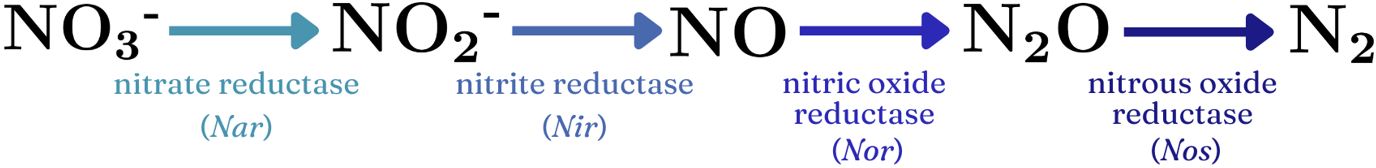
\includegraphics[width=6.5in,height=\textheight]{images/clipboard-3756250656.png}

Each microorganism in this pathway has a specific enzyme that catalyzes
one particular reaction in the sequence, with the collective result of
denitrification.\footnote{More on this later. Denitrification is an
  important aspect of the role that sediment microbes in oyster beds
  play as water purifiers.} Dr.~Lawrence Pomeroy describes such
microbial community behaviors as ``external digestive processes
{[}which{]} provide shared benefits for motile bacteria'' (Pomeroy et
al., n.d.). Dr.~Farooq Azam simplifies this further, calling microbial
communities the ``ultimate swimming stomachs'' (Pomeroy et al., n.d.).

While the typical depiction of the food chain is a pyramid with plants
at the base, topped by primary, secondary, and tertiary consumers--much
of the available energy in our food webs derives from microbes. The
microbial loop begins with photosynthetic bacterioplankton
(i.e.~bacteria and archaeans that drift through the water column)
(Pomeroy et al., n.d.). Much like the photosynthetic process that we
visualize occurring in plant life, these bacterioplankton take in
sunlight energy (and sometimes heat energy; this process is known as
chemosynthesis) to form organic compounds from inorganic compounds and
molecules (Pomeroy et al., n.d.). One example of the microbial loop
could look like this: bacterioplankton are eaten by microflagellates
(less than 0.002 millimeters big), who are eaten by ciliates (ex.
paramecium, usually 0.02-0.2 millimeters), who are eaten by copepods
(1-2 millimeters, typically) and mezozooplankton (mid-size animal
plankton, 0.2-20 millimeters). It is at this point that fish larvae
enter the picture as predators and the food chain continues onto a
macroscopic scale. However, sometimes the grand microbial loop is
short-circuited; organisms like oysters and krill are filter-feeders,
casting out mucus nets and capturing a wide range of microorganisms as
they pump seawater through their gills. Connecting the so-called ``end''
of the microbial loop back to its ``beginning,'' some microbial species
break down decaying organisms and detritus, returning matter back to the
water column in the form of minerals. These minerals may become organic
compounds, thanks to photosynthetic organisms like our friend, the
bacterioplankton.

In summary, microbes are diverse and abundant. Their community actions
provide us with nutrients we need, and they provide the ecosystems we
are reliant upon with necessary nutrients. So when we talk about the
factors at play regulating ecological systems, when we talk about the
cycling of nutrients between earth, water, sky, and us, it does us well
to acknowledge that the drivers of biological processes are
microorganisms. It's a microbial world; we're just living in it.

\section{Introduction to oyster
farming}\label{introduction-to-oyster-farming}

As we face the deleterious ecological impacts of current industrial and
agricultural production methods, oyster aquaculture has been proposed as
part of a food system reimagined to have greater sustainability. Not
only does oyster cultivation bypass common agricultural issues like land
scarcity; farming oysters can provide benefits to the health of the
marine ecosystems to which they are native. These potential benefits
include enhanced water quality, habitat provision to other marine
species, and storm surge protection (Stevens et al. 2024).

\begin{wrapfigure}{l}{0.5\textwidth}
  \vspace{-\baselineskip}
  \centering
    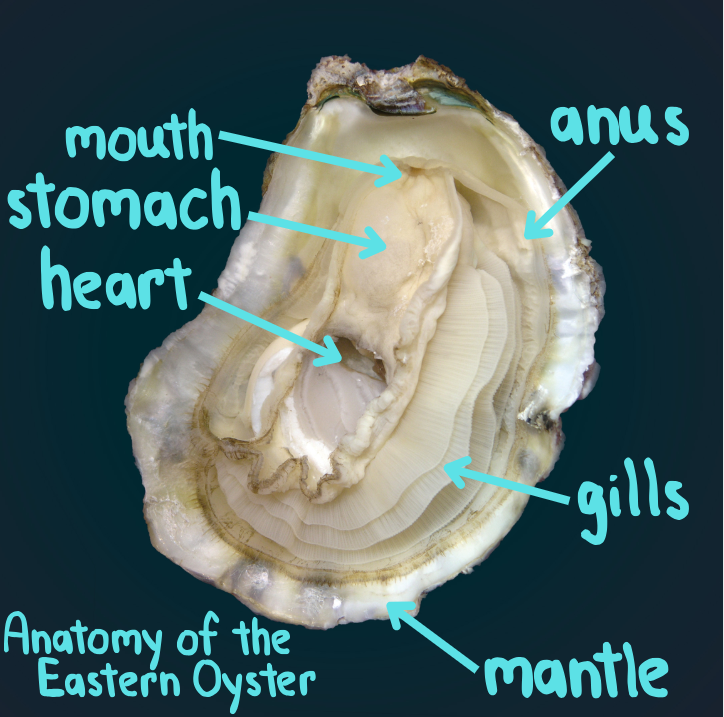
\includegraphics[width=\linewidth]{images/clipboard-2987364097.png}
  \caption{Selected Anatomy of an Eastern Oyster, *Crossastrea virginica*. (Source: https://www.mdsg.umd.edu/lesson-plans/eastern-oyster-education)}
  \vspace{-\baselineskip}
\end{wrapfigure}

(\^{}\^{}\^{}need help getting text to wrap here.)

Oysters are filter-feeders. They filter \textasciitilde50 gallons of
seawater per day, taking in algae and large plankton through their gills
while smaller plankton and water pass through. The organic matter
retained by the oyster is then either ingested, passing through the
oyster's digestive tract to be excreted as feces, or rejected by the
oyster, wrapped in a mucosal lining and deposited into the sediment as
pseudofeces.

\begin{itemize}
\tightlist
\item
  nitrogen loading responsible for biodiversity declines (Ray and
  Fulweiler 2021) pg 1
\end{itemize}

\section{Theory \#1: Oysters enhance the biodiversity and composition of
microbial communities in the
seafloor.}\label{theory-1-oysters-enhance-the-biodiversity-and-composition-of-microbial-communities-in-the-seafloor.}

Oysters themselves filter water by taking in plankton while seawater
passes through their gills, however, the perhaps greater source of
denitrification in the relationship between oysters and their
environment is the microbial communities in their biodeposits (poop).
The abundance of urea and ammonia increases microbial growth. Most
abundant in these samples were proteobacteria, firmicutes,
bacteriodetes, and actinobacteria. Notably, these are all denitrifiers.
Some studies showed underwhelming changes to the microbial community in
the presence and absence of oyster farming. The one paper on different
methods within the Mass Bay (I think it was the Northeastern paper?)
found that hanging oysters (grown suspended in the water column) did not
impact the soil communities as the oysters were not in contact with the
ground. I think there was a study that said older oyster beds had
different microbiomes compared to younger ones, measured at year 3, 5,
and 7. One paper took into consideration the potential for pathogenic
microbes to humans coming from oysters. This paper (\#5) found that
\emph{Vibrio} species were found in the oyster sediments (\emph{Vibrio}
being associated with food-borne illnesses stemming from seafood).
However, the \emph{Vibrio} were not the pathogenic strains. The
\emph{Vibrio} present in the samples were determined to not be harmful
to human health.

Oysters promote biodiverse microbial communities by providing microbes
in the marine sediments with diverse nutrients. Some bacteria species
(some denitrifiers?) need trace metals to survive. Oysters provide these
to the sediment.

Although it may be easier to understand that oysters themselves are the
big denitrifiers, one of the papers argue that the sediment microbes are
doing more of the work. Similarly to how there is emphasis in
agriculture on creating living soils, on soil as a community that pulls
in CO2 from the atmosphere instead of just seeing plants as the main
carbon sinks, the marine floor can be seen as a living sediment, where
decaying matter is broken down by microbes for the nutrients to be
sequestered or recycled.

\begin{itemize}
\item
  ``nitrate reductase requires a Molybdenum protein co-factor for
  reducing nitrate to nitrite'' (Stevens et al. 2024)
\item
  ``nitrous oxide reductase requires Cu for reducing nitrous oxide
  (N\textsubscript{2}O) to N\textsubscript{2}'' (Stevens et al. 2024)
\item
  concentration of iron has sig. role in how microbes cycle P (Stevens
  et al. 2024) makes me need to go back to biogeochem paper to learn
  about P cycling
\end{itemize}

\section{Theory \#2: Oysters stimulate increased denitrification by
sediment
microbiota.}\label{theory-2-oysters-stimulate-increased-denitrification-by-sediment-microbiota.}

Oyster sediment microbes boost the recycling, cycling, and sequestering
of many nutrients in the water column, including nitrogen, phosphorous,
and silicon. This can help to combat eutrophication and climate change.
Industrial and agriculture production often releases excess nutrients,
like the three mentioned above, into bodies of water in the form of
fuel, fertilizer, and waste run-off. The papers contradict each other
with how pronounced this impact is. Some did not even find the
difference in eutrophication to be statistically significant. I am
curious how they separate the impact of microbes living in and on
oysters from those in the sediments. Just a thought. Sediment microbes,
like actinobacteria and proteobacteria are part of the denitrification
process.

Here's the pathway: nutrient loading on aquatic system - probably from
anthropogenic activity. Then, this stimulates an increase in the
abundance of many photosynthetic organisms, like cyanobacteria. All the
time, decaying matter and detritus is falling through the water column
in the form of marine snow. When oysters ``catch'' plankton and other
microbes and algae, they are pulled out from the water column, boosting
water clarity. The seafloor is, ideally covered in decay and also
microbes. It is a place of regeneration, of recycling. When sediment
microbes take in nitrogen paired with organic material (usually it will
be in the form of ammonia or urea, although neither of those are
organics?? But are they just with carbon anyway?) microbes break the
bonds between nitrogen and hydrogen, returning hydrogen to the water
column? At some points, our nitrogens in the process of denitrification
are paired with oxygens but the oxygens are eventually returned to the
water column. Close to the end of the process of denitrification,
nitrous oxide is created. Nitrous oxide is a harmful greenhouse gas,
however, the amounts released from sediment denitrification are very
small. The Fulweiler meta-analysis suggests that the amount of nitrous
oxide released is negligible. This would be a good place to put the Ray
and Fulweiler nutrient flux diagram

Oyster poop microbes remineralize unstable nitrogen compounds (urea,
ammonia, nitrate, nitrite, nitric oxide, nitrous oxide), returning them
to the water column as N\textsubscript{2}. Diatom nitrogen makes up like
70\% of our atmosphere and gas rises so a lot of the N\textsubscript{2}
is recycled back into the air. Kind of cool that we are all breathing
matter that had its energy spent and has been recycled billions of time.
From death back unto life, or something like that.

So to sum it up, oyster sediment bacteria improve water quality and
combat eutrophication. Now I am realizing that I need to learn more
about how they actually combat eutrophication and mitigate global
warming. I think I've mentioned sequestering, but do they really
sequester? Maybe I'm getting carbon cycle and nitrogen cycle confused.

\begin{itemize}
\item
  17/45 studies report fluxes from oysters, 31/45 report fluxes from
  sediments (Ray and Fulweiler 2021), pg 1
\item
  ``sediments beneath oysters return significantly more
  NH\textsubscript{4}\textsuperscript{+} to the water column than bare
  sediments'' (Ray and Fulweiler 2021), pg. 2, 1st col, oysters have
  highly-variable effect on NO\textsubscript{x} fluxes between studies,
  in contrast
\item
  ``\,``oysters also have a strong effect on sediment phosphate
  regeneration'' (Ray and Fulweiler 2021), si unclear
\item
  ``Stimulation of sediment denitrification and denitrification in
  oysters can permenantly remove excess N from coatal systems, reducting
  the impact of europhication.'' (Ray and Fulweiler 2021), pg 2`
\item
  check pg 3z - effect on primary production. promote nitrogen
  recycling, but add back to system? How does this combat
  denitrification?
\item
  Seems that oysters do not have a net positive ability related to
  sequestering carbon. Installing oyster aquacutlutre initially
  increases sediment CO\textsubscript{2} and CH\textsubscript{4}
  release, before returning to baseline. This is good compared to more
  typical forms of raising protein because for example, cow corn
  monoculture releases hella GHGs from soils. But there are limited
  studies on the impact of oyster aquacutluutre on GHG emissions. I am
  left wondering about the strength of the one study discussed in the
  Ray paper. Also, do oysters themselves release GHGs?* Are there other
  pieces of oyster awauculture that release GHGs? Restoration projects
  are underway; should they be?
\item
  *Omg. Discussed in next paragraph. pg 4 column 2 of ray and fulweiler
\end{itemize}

\section{Trade-offs}\label{trade-offs}

I attended a Cornell presentation session with my dad on the NYC campus
many years ago. One of the presentation discussed the planning of
coastal cities, with a focus on Hudson Bay oysters. I knew from this
experience that oysters were once prevalent in the Hudson, but
populations were decimated in the nineteenth and early twentieth
centuries. I heard about projects to build up the oyster populations for
storm surge protection (coral reefs work similarly and it is the same
concept as keeping a ground cover on cropland to prevent erosion (and
dust bowls!). Barnacle life slows the advance of oncoming waves.) and to
improve water quality through their filtration properties. This sounded
like a wonderful solution and something that should be widely
implemented. However, the studies I have read (not even my actual
research project, just learning about other people's work) has made me
wary of trade-offs to ``sustainable'' solutions. For example, the
denitrification by sediment microbes is an intermediate, and therefore
leaky process. Before nitrates and nitrites (NOₓ groups) are fully
reduced to N₂, they become nitrous oxide molecules (a potent greenhouse
gas), some of which escape into the atmosphere. This happens on a much
smaller scale than anthropogenic greenhouse gas emission, but it is
still happening. The paper that~

increasing dinoflagellate growth

\subsection{Conclusion}\label{conclusion}

\subsection*{Citations}\label{citations}
\addcontentsline{toc}{subsection}{Citations}

\phantomsection\label{refs}
\begin{CSLReferences}{1}{0}
\bibitem[\citeproctext]{ref-denitrif}
{``Denitrifying Bacterium - an Overview \textbar{} ScienceDirect
Topics.''} n.d.
\url{https://www.sciencedirect.com/topics/biochemistry-genetics-and-molecular-biology/denitrifying-bacterium}.

\bibitem[\citeproctext]{ref-pomeroy}
Pomeroy, Lawrence R., Peter J. leB Williams, Farooq Azam, and John E.
Hobbie. n.d. {``The Microbial Loop \textbar{} Oceanography.''}
\url{https://tos.org/oceanography/article/the-microbial-loop}.

\bibitem[\citeproctext]{ref-ray2021}
Ray, Nicholas E., and Robinson W. Fulweiler. 2021. {``Meta-Analysis of
Oyster Impacts on Coastal Biogeochemistry.''} \emph{Nature
Sustainability} 4 (3): 261--69.
\url{https://doi.org/10.1038/s41893-020-00644-9}.

\bibitem[\citeproctext]{ref-stevens2024}
Stevens, Joshua T. E., Nicholas E. Ray, Alia N. Al-Haj, Robinson W.
Fulweiler, and Priyanka Roy Chowdhury. 2024. {``Oyster Aquaculture
Enhances Sediment Microbial Diversity: Insights from a Multi-Omics
Study.''} \emph{Aquaculture Environment Interactions} 16 (December):
283--301. \url{https://doi.org/10.3354/aei00484}.

\end{CSLReferences}

\end{document}
